% Options for packages loaded elsewhere
\PassOptionsToPackage{unicode}{hyperref}
\PassOptionsToPackage{hyphens}{url}
\documentclass[
  11pt,
]{report}
\usepackage{xcolor}
\usepackage[margin=1in]{geometry}
\usepackage{amsmath,amssymb}
\setcounter{secnumdepth}{5}
\usepackage{iftex}
\ifPDFTeX
  \usepackage[T1]{fontenc}
  \usepackage[utf8]{inputenc}
  \usepackage{textcomp} % provide euro and other symbols
\else % if luatex or xetex
  \usepackage{unicode-math} % this also loads fontspec
  \defaultfontfeatures{Scale=MatchLowercase}
  \defaultfontfeatures[\rmfamily]{Ligatures=TeX,Scale=1}
\fi
\usepackage{lmodern}
\ifPDFTeX\else
  % xetex/luatex font selection
\fi
% Use upquote if available, for straight quotes in verbatim environments
\IfFileExists{upquote.sty}{\usepackage{upquote}}{}
\IfFileExists{microtype.sty}{% use microtype if available
  \usepackage[]{microtype}
  \UseMicrotypeSet[protrusion]{basicmath} % disable protrusion for tt fonts
}{}
\makeatletter
\@ifundefined{KOMAClassName}{% if non-KOMA class
  \IfFileExists{parskip.sty}{%
    \usepackage{parskip}
  }{% else
    \setlength{\parindent}{0pt}
    \setlength{\parskip}{6pt plus 2pt minus 1pt}}
}{% if KOMA class
  \KOMAoptions{parskip=half}}
\makeatother
\usepackage{longtable,booktabs,array}
\usepackage{calc} % for calculating minipage widths
% Correct order of tables after \paragraph or \subparagraph
\usepackage{etoolbox}
\makeatletter
\patchcmd\longtable{\par}{\if@noskipsec\mbox{}\fi\par}{}{}
\makeatother
% Allow footnotes in longtable head/foot
\IfFileExists{footnotehyper.sty}{\usepackage{footnotehyper}}{\usepackage{footnote}}
\makesavenoteenv{longtable}
\usepackage{graphicx}
\makeatletter
\newsavebox\pandoc@box
\newcommand*\pandocbounded[1]{% scales image to fit in text height/width
  \sbox\pandoc@box{#1}%
  \Gscale@div\@tempa{\textheight}{\dimexpr\ht\pandoc@box+\dp\pandoc@box\relax}%
  \Gscale@div\@tempb{\linewidth}{\wd\pandoc@box}%
  \ifdim\@tempb\p@<\@tempa\p@\let\@tempa\@tempb\fi% select the smaller of both
  \ifdim\@tempa\p@<\p@\scalebox{\@tempa}{\usebox\pandoc@box}%
  \else\usebox{\pandoc@box}%
  \fi%
}
% Set default figure placement to htbp
\def\fps@figure{htbp}
\makeatother
\setlength{\emergencystretch}{3em} % prevent overfull lines
\providecommand{\tightlist}{%
  \setlength{\itemsep}{0pt}\setlength{\parskip}{0pt}}
\usepackage{bookmark}
\IfFileExists{xurl.sty}{\usepackage{xurl}}{} % add URL line breaks if available
\urlstyle{same}
\hypersetup{
  pdftitle={MC SMC+VAS Baseline Analysis Bauchi State, Nigeria -- 2025},
  pdfauthor={Malaria Consortium},
  hidelinks,
  pdfcreator={LaTeX via pandoc}}

\title{\textbf{MC SMC+VAS Baseline Analysis}\\
\emph{Bauchi State, Nigeria -- 2025}}
\author{Malaria Consortium}
\date{June 23, 2025}

\begin{document}
\maketitle

{
\setcounter{tocdepth}{1}
\tableofcontents
}
\chapter{Introduction}\label{introduction}

Malaria Consortium is one of the world's leading non-profit
organizations specializing in the prevention, control, and treatment of
malaria and other communicable diseases among vulnerable populations
across Africa and Asia. In Nigeria, the organization is at the forefront
of supporting the delivery of high-impact child survival interventions
such as \textbf{Seasonal Malaria Chemoprevention (SMC)} and
\textbf{Vitamin A Supplementation (VAS)}, both proven strategies for
reducing morbidity and mortality among children under five years of age.

Despite national guidelines recommending biannual high-dose VAS for
children 6--59 months, VAS coverage in Nigeria remains suboptimal, with
national estimates at just 45\% (NDHS 2018), compared to the high
coverage typically achieved by SMC campaigns (often \textgreater95\%).
The periodic \textbf{Maternal, Newborn and Child Health Week (MNCHW)}
campaigns serve as the main platform for delivering VAS and other key
health and nutrition interventions; however, significant gaps in
coverage persist, especially among hard-to-reach children.

In response to these challenges, and building on evidence from
implementation research conducted in Sokoto and Bauchi States, Malaria
Consortium, with support from GiveWell---has launched a large-scale
evaluation to assess the \textbf{effectiveness and impact of integrating
VAS delivery into SMC campaigns} in Bauchi and Niger states. This
innovative approach aims to leverage the high reach and acceptability of
SMC campaigns to improve the uptake of VAS, using a door-to-door
delivery model. The strategy also involves removing VAS from the MNCHW
package during the first biannual campaign of 2025, to prevent
duplication and assess potential effects on the uptake of other MNCHW
interventions.

The present baseline survey, conducted in April 2025 in Bauchi State, is
part of a convergent mixed-methods evaluation designed to measure:

\begin{itemize}
\tightlist
\item
  The effectiveness (coverage and quality) of VAS co-implementation with
  SMC at scale;
\item
  Whether integrating VAS with SMC affects the coverage and uptake of
  other key MNCHW interventions;
\item
  Health worker and policy maker perceptions regarding the integration
  and any unintended effects on service demand.
\end{itemize}

The study targets children under five years old (with eligibility
criteria specified for both SMC and VAS), as well as female caregivers
of childbearing age (15--49 years) in sampled households across Bauchi
State. The evidence generated will inform national policy and provide
operational lessons for the scale-up of integrated child survival
campaigns in Nigeria and beyond.

\chapter{Study Objectives}\label{study-objectives}

\section{Aim of the Study}\label{aim-of-the-study}

The overarching aim of this baseline evaluation is to generate robust
empirical evidence regarding the effectiveness, operational feasibility,
and community acceptability of integrating \textbf{Vitamin A
Supplementation (VAS)} into \textbf{Seasonal Malaria Chemoprevention
(SMC)} campaigns in Bauchi State, Nigeria. The findings of this study
are intended to inform national and sub-national policy decisions, as
well as contribute to the global knowledge base on integrated child
health interventions in malaria-endemic settings.

\section{Specific Objectives}\label{specific-objectives}

This study is structured around the following primary and secondary
objectives:

\subsection{Primary Objectives}\label{primary-objectives}

\begin{enumerate}
\def\labelenumi{\arabic{enumi}.}
\item
  \textbf{To determine the effect of integrating VAS with SMC on the
  uptake of other key Maternal, Newborn, and Child Health Week (MNCHW)
  interventions.}\\
  This objective focuses on quantifying the extent to which integrated
  delivery influences coverage of core MNCHW services such as deworming,
  immunization, and nutritional screening.
\item
  \textbf{To assess health workers' and policy makers' perceptions of
  the effect of removing VAS from MNCHW on the demand for and uptake of
  MNCHW interventions.}\\
  This includes exploring the anticipated and observed impacts on
  community engagement, service delivery, and health system operations
  from the perspective of frontline implementers and decision-makers.
\item
  \textbf{To determine the coverage of vitamin A following its
  integration with SMC.}\\
  The study aims to estimate VAS coverage rates among eligible children
  both prior to and following the integrated campaign, thereby
  establishing a baseline for future impact evaluation.
\item
  \textbf{To monitor the coverage and quality of SMC following
  integration with VAS.}\\
  This objective seeks to ensure that integration does not compromise
  the effectiveness or operational quality of SMC delivery.
\end{enumerate}

\subsection{Secondary Objectives}\label{secondary-objectives}

\begin{enumerate}
\def\labelenumi{\arabic{enumi}.}
\item
  \textbf{To identify barriers and facilitators to the uptake of VAS and
  other MNCHW interventions.}\\
  By mapping individual, community, and health system factors, the study
  seeks to understand why some eligible populations remain unreached or
  are sub-optimally served.
\item
  \textbf{To assess community awareness and perceptions of integrated
  campaign models.}\\
  This objective examines knowledge, attitudes, and practices (KAP)
  among caregivers, as well as perceived acceptability and trust in the
  new delivery approach.
\end{enumerate}

\section{Research Questions}\label{research-questions}

Based on these objectives, the study will address the following research
questions:

\begin{itemize}
\tightlist
\item
  What is the baseline coverage of VAS, SMC, deworming, immunization,
  and nutritional screening among target populations in Bauchi State?
\item
  What are the perceptions of health workers, policy makers, and
  caregivers regarding the integration of VAS into SMC campaigns?
\item
  What operational or contextual barriers hinder the effective delivery
  and uptake of integrated services?
\item
  How does integration affect the quality, completeness, and equity of
  service delivery for both VAS and SMC?
\item
  What is the level of community awareness of integrated campaigns, and
  what factors shape their participation?
\end{itemize}

\section{Significance of the Study}\label{significance-of-the-study}

This evaluation is expected to provide critical insights for optimizing
child health delivery strategies in Nigeria and similar settings. The
evidence generated will not only inform local implementation but may
also contribute to national and global policy discussions on integrated
service delivery for child survival interventions.

\chapter{Study Design and Methods}\label{study-design-and-methods}

\section{Study Design}\label{study-design}

This baseline evaluation employs a \textbf{convergent mixed-methods
design}, integrating both quantitative and qualitative approaches to
achieve comprehensive insights:

\begin{itemize}
\item
  \textbf{Quantitative Component:}\\
  A cross-sectional household survey was conducted in April 2025 among
  randomly sampled households across all 20 LGAs of Bauchi State. Data
  collection targeted children aged 6--59 months and women of
  childbearing age (15--49 years). The survey gathered detailed
  information on coverage of VAS, SMC, deworming, immunization, and
  nutrition interventions, as well as household and caregiver
  characteristics.
\item
  \textbf{Qualitative Component:}\\
  Key Informant Interviews (KIIs) and Focus Group Discussions (FGDs)
  were held with health workers, policy makers, and community leaders to
  explore perceptions regarding the integration of VAS and SMC,
  potential effects on other services, and barriers to uptake.\\
  The qualitative strand aims to complement and explain quantitative
  findings, providing context for observed coverage rates and
  health-seeking behavior.
\end{itemize}

\section{Sampling and Analysis
Methods}\label{sampling-and-analysis-methods}

\subsection{Sampling Approach}\label{sampling-approach}

The study employed a rigorous multi-stage stratified cluster sampling
methodology to ensure that the findings would be generalizable across
Bauchi State's diverse population. In the first stage, all twenty Local
Government Areas (LGAs) within the state were included in the sampling
frame, ensuring statewide representativeness. Subsequently, wards within
each LGA were stratified according to urban and rural status, drawing
upon the INEC polling unit directory and LGA population projections to
guide proportional allocation.

Within each selected ward, a random sampling technique was used to
select communities, with the probability of selection proportional to
the size of the community population. Systematic random sampling was
then utilized to identify households within each selected community. To
be eligible, households were required to have at least one child aged
6--59 months or a woman of childbearing age (15--49 years).

The minimum required sample size for each LGA was determined using
established statistical formulas for cluster surveys. The calculations
incorporated assumptions regarding the expected prevalence of key
indicators, a design effect of 2.0 to account for intra-cluster
correlation, and the application of a finite population correction where
appropriate. Ultimately, the study achieved a sample of approximately
8,064 children and a comparable number of women of childbearing age,
allowing for precise estimation of primary outcomes and adequate
statistical power for subgroup analyses.

\section{Data Collection Procedures}\label{data-collection-procedures}

Data were collected by trained field teams employing structured
electronic questionnaires administered via mobile tablets. The
questionnaires covered a wide array of topics, including household
composition, child health interventions (e.g., SMC, VAS, deworming, and
immunization), women's health services, and barriers to service
utilization. To enhance data quality and reduce potential bias, regular
field supervision was conducted, GPS-enabled spot checks were
implemented, and daily reviews of completed questionnaires took place.

In addition to quantitative data collection, qualitative information was
gathered through Key Informant Interviews (KIIs) and Focus Group
Discussions (FGDs). KIIs were conducted with policy-makers, health
managers, and program coordinators at both LGA and state levels. FGDs
were held with caregivers, community leaders, and frontline health
workers, guided by thematic areas informed by the WaterAid Gender
Analysis Guide and the objectives of SMC/VAS integration.

\section{Analytical Methods}\label{analytical-methods}

Quantitative data analysis was conducted using R and Microsoft Power BI.
Descriptive statistics, including means, proportions, and 95\%
confidence intervals, were computed for all key indicators. Comparative
analyses were conducted by disaggregating outcomes by LGA, educational
attainment, and other sociodemographic variables. Associations between
variables were evaluated using Pearson's chi-squared tests, with
Cramer's V calculated to assess the strength of observed relationships.
Where applicable, sampling weights were applied to adjust for the
multi-stage design and non-response.

Qualitative data analysis was performed using NVivo software.
Transcripts from KIIs and FGDs were subjected to thematic analysis, with
codes and themes developed inductively and deductively based on the
study objectives and interview guides. Findings from the qualitative
analysis were triangulated with quantitative results to provide a richer
understanding of patterns and contextual drivers underlying service
uptake and coverage.

\section{Ethical Considerations}\label{ethical-considerations}

Ethical approval for the study was obtained from relevant institutional
review boards. Written informed consent was sought from all study
participants prior to data collection. All data were stored securely and
anonymized prior to analysis to ensure confidentiality and privacy.

\section{Study Limitations}\label{study-limitations}

This study's cross-sectional design provides a snapshot of coverage and
perceptions at a single point in time, which may not capture seasonal or
temporal variations. While every effort was made to validate responses
through health card verification and supervisory checks, there remains a
possibility of recall bias and social desirability bias in self-reported
indicators.

\chapter{Results}\label{results}

\section{Demographic Profile of
Respondents}\label{demographic-profile-of-respondents}

A total of 8,064 households were surveyed across all 20 Local Government
Areas (LGAs) of Bauchi State. The distribution of respondents was broad
and representative, with no single LGA accounting for more than 6.2\% of
the sample. This even distribution enhances the generalizability of
findings and reduces the risk of location-based sampling bias. The
largest numbers of households were recorded in Alkaleri, Bauchi,
Katagum, and Zaki LGAs, each contributing over 6\% of the total sample,
while other LGAs such as Bogoro, Dass, Giade, Jama'are, Kirfi, and Warji
contributed approximately 4\% each. This proportional allocation
underscores the study's intention to capture the heterogeneity of
population structures, access to health services, and potential
differences in intervention coverage across the state.

\textbf{Table 1: Distribution of LGAs}

\begin{longtable}[]{@{}lrr@{}}
\toprule\noalign{}
LGA & Frequency & Percent \\
\midrule\noalign{}
\endhead
\bottomrule\noalign{}
\endlastfoot
Alkaleri & 499 & 6.2 \\
Bauchi & 502 & 6.2 \\
Bogoro & 325 & 4.0 \\
DAMBAM & 398 & 4.9 \\
Darazo & 418 & 5.2 \\
Dass & 325 & 4.0 \\
Gamawa & 449 & 5.6 \\
Ganjuwa & 400 & 5.0 \\
Giade & 325 & 4.0 \\
Itas/Gadau & 400 & 5.0 \\
Jama'are & 325 & 4.0 \\
Katagum & 501 & 6.2 \\
Kirfi & 323 & 4.0 \\
Misau & 400 & 5.0 \\
Ningi & 400 & 5.0 \\
Shira & 474 & 5.9 \\
Tafawa-Balewa & 400 & 5.0 \\
Toro & 425 & 5.3 \\
Warji & 325 & 4.0 \\
Zaki & 450 & 5.6 \\
\textbf{Total} & 8,064 & 100.0 \\
\end{longtable}

\pandocbounded{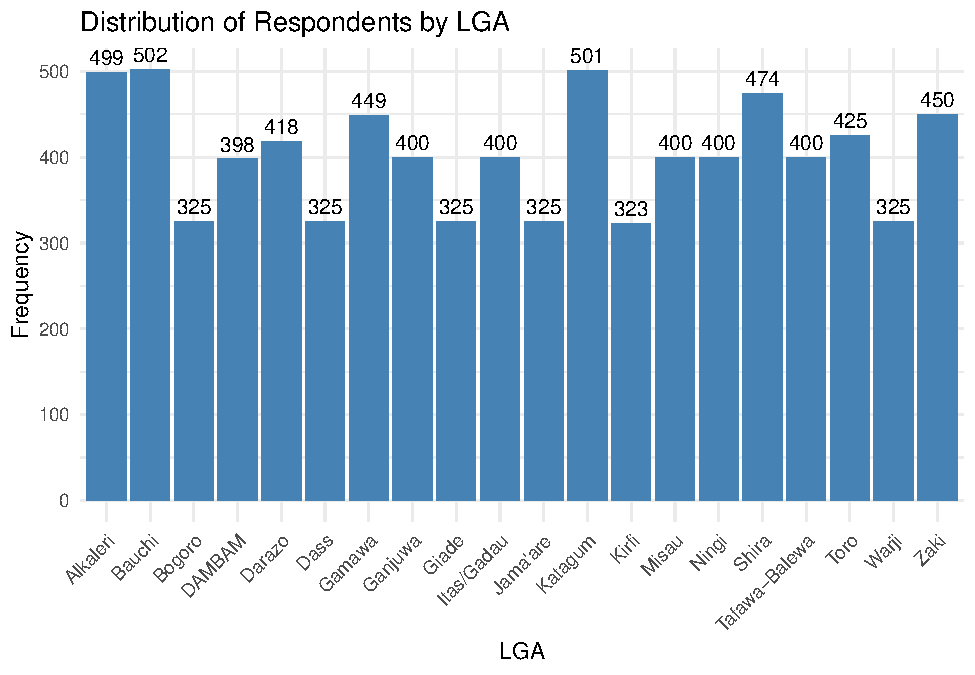
\includegraphics[keepaspectratio]{MC-SMCVAS-Baseline-Analysis_files/figure-latex/unnamed-chunk-3-1.pdf}}
\#\# 2. Household and Population Structure

The surveyed households exhibited moderate to high fertility and complex
family structures, which is common in northern Nigeria's rural and
semi-urban areas. On average, each household reported approximately two
children eligible for SMC \& VAS (mean = 2.01), and about two children
not eligible for SMC (mean = 1.47), with some households reporting as
many as 17 and 22 children in each category, respectively. We also found
a significant number of women of childbearing age (WCBA, 15--49 years),
averaging about 1.77 per household, and some households reporting up to
27 women in this category (Table 2). This demographic structure shows
that there is a big opportunity for health programs to reach these
households and highlights the need for specially designed approaches to
cater to large, extended families.

\begin{itemize}
\tightlist
\item
  \textbf{Children eligible for SMC \& VAS:} The mean number per
  household was 2.01 (range 0--17).
\item
  \textbf{Children not eligible for SMC:} The mean was 1.47 per
  household (range 0--22).
\item
  \textbf{Women of childbearing age (WCBA):} The mean per household was
  1.77 (range 0--27).
\end{itemize}

\textbf{Table 2: Distribution of Children and WCBA per Household}

\begin{longtable}[]{@{}lllll@{}}
\toprule\noalign{}
Variable & Mean & SD & Minimum & Maximum \\
\midrule\noalign{}
\endhead
\bottomrule\noalign{}
\endlastfoot
Children eligible SMC & 2.01 & --- & 0 & 17 \\
Children non-SMC & 1.47 & --- & 0 & 22 \\
WCBA (15--49 years) & 1.77 & --- & 0 & 27 \\
\end{longtable}

\emph{Note: SD not available from summary provided.}

\begin{center}\rule{0.5\linewidth}{0.5pt}\end{center}

\section{3. Age Distribution of Key
Respondents}\label{age-distribution-of-key-respondents}

The mean age of selected women of childbearing age (WCBA) was 27.7
years, with the age range spanning from 15 to 49 years. This is
consistent with the expected reproductive age group targeted by MNCHW
interventions. The mean age of household heads was 41.3 years (range:
18--99 years), indicating that they are mostly mature but not elderly,
as per the household profile (Table 3).

\textbf{Table 3: Age Distribution of Selected Women and Household Heads}

\begin{longtable}[]{@{}llll@{}}
\toprule\noalign{}
Group & Mean Age (years) & Min & Max \\
\midrule\noalign{}
\endhead
\bottomrule\noalign{}
\endlastfoot
Selected WCBA & 27.7 & 15 & 49 \\
Household Head & 41.3 & 18 & 99 \\
\end{longtable}

\section{4. Sex of Household Head}\label{sex-of-household-head}

Males predominated as heads of household, accounting for 97.3\% (n =
7,843), while females constituted only 2.7\% (n = 221).

\textbf{Table 4: Sex Distribution of Household Heads}

\begin{longtable}[]{@{}lll@{}}
\toprule\noalign{}
Sex & Frequency & Percent \\
\midrule\noalign{}
\endhead
\bottomrule\noalign{}
\endlastfoot
Male & 7,843 & 97.3\% \\
Female & 221 & 2.7\% \\
\end{longtable}

\pandocbounded{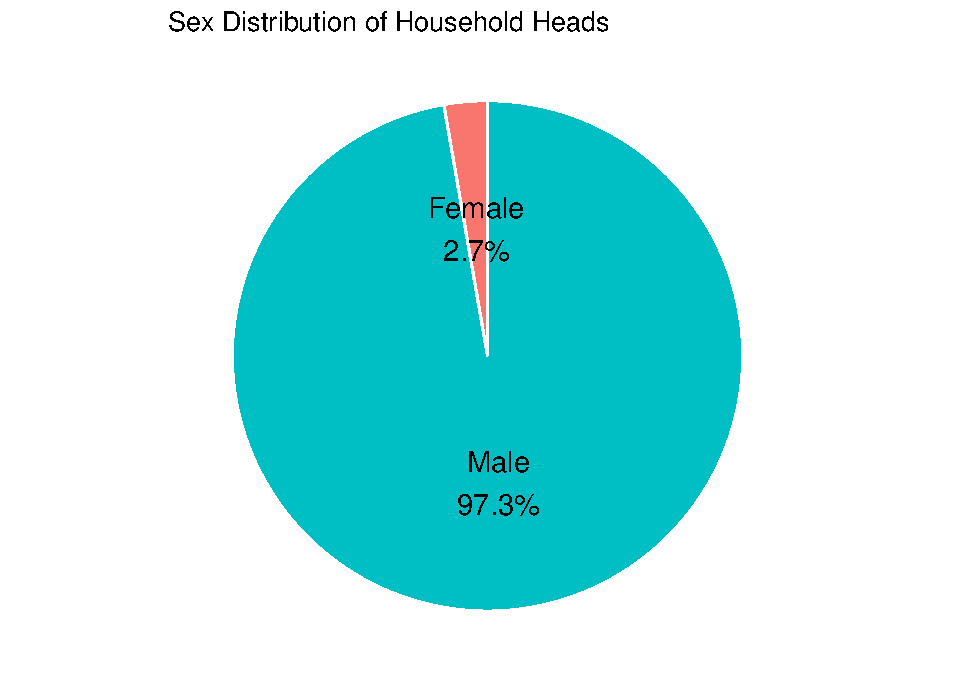
\includegraphics[keepaspectratio]{MC-SMCVAS-Baseline-Analysis_files/figure-latex/unnamed-chunk-4-1.pdf}}
\#\# 5. Employment and Occupation of Household Head

A substantial proportion of the surveyed household heads (73.9\%) were
self-employed, mainly in informal jobs like farming and petty trading.
Formal jobs are less common (12.9\%), and 13.2\% are unemployed. The
most common occupation is farming (41.0\%), followed by trading
(18.8\%), civil service (8.3\%), cattle rearing (5.2\%), and technical
trades (3.3\%). Fishing is rare (0.7\%). These results highlight the
area's focus on agriculture and suggest that changes in seasons could
influence participation in health campaigns.

\textbf{Table 5: Occupation of Household Head}

\begin{longtable}[]{@{}lll@{}}
\toprule\noalign{}
HH\_Occupation & Percent (\%) & Frequency \\
\midrule\noalign{}
\endhead
\bottomrule\noalign{}
\endlastfoot
Farming & 41.0 & 3310 \\
Trading & 18.8 & 1516 \\
Civil Servant & 8.3 & 669 \\
Cattle rearing & 5.2 & 418 \\
Technician & 3.3 & 270 \\
Fishing & 0.7 & 59 \\
Other/Unspecified & 9.4 & 758 \\
\end{longtable}

\textbf{Table 6: Employment of Household Head}

\begin{longtable}[]{@{}lll@{}}
\toprule\noalign{}
HHH\_Employment & Percent (\%) & Frequency \\
\midrule\noalign{}
\endhead
\bottomrule\noalign{}
\endlastfoot
Employment & 12.9 & 1040 \\
Self-employment & 73.9 & 5960 \\
Unemployed & 13.2 & 1064 \\
\end{longtable}

\pandocbounded{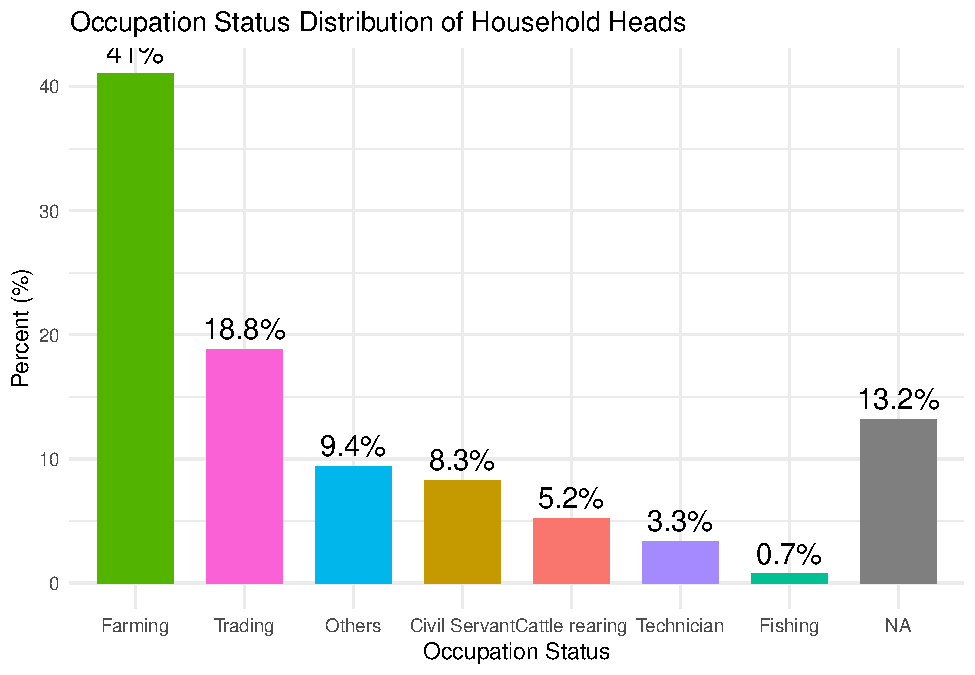
\includegraphics[keepaspectratio]{MC-SMCVAS-Baseline-Analysis_files/figure-latex/unnamed-chunk-6-1.pdf}}
\#\# 6. Educational Status of Household Head Slightly more than half
(53.2\%) of household heads had ever attended school, whereas 46.8\% had
never attended any formal education. Among those who had some education,
secondary (22.9\%) and higher/tertiary education (14.9\%) were most
frequently reported, with a smaller proportion attaining primary
(13.1\%) or pre-primary education (1.2\%). Notably, 1.0\% of respondents
were unable to specify the highest education level of the household head
(Table 5). The high proportion of uneducated household heads signals
potential challenges in communication and comprehension of health
messages, which could in turn influence uptake of SMC, VAS, and other
MNCHW interventions. However, the substantial presence of secondary and
tertiary education suggests opportunities for leveraging literate
household members as health promotion champions.

\section{Education Level of Household
Heads}\label{education-level-of-household-heads}

\begin{longtable}[]{@{}lll@{}}
\toprule\noalign{}
Education Level & Frequency & Percent (\%) \\
\midrule\noalign{}
\endhead
\bottomrule\noalign{}
\endlastfoot
Don't Know & 80 & 1.0 \\
Higher & 1205 & 14.9 \\
Pre-primary/kindergarten & 94 & 1.2 \\
Primary & 1060 & 13.1 \\
Secondary & 1848 & 22.9 \\
Unspecified (NA) & 3777 & 46.8 \\
\end{longtable}

\pandocbounded{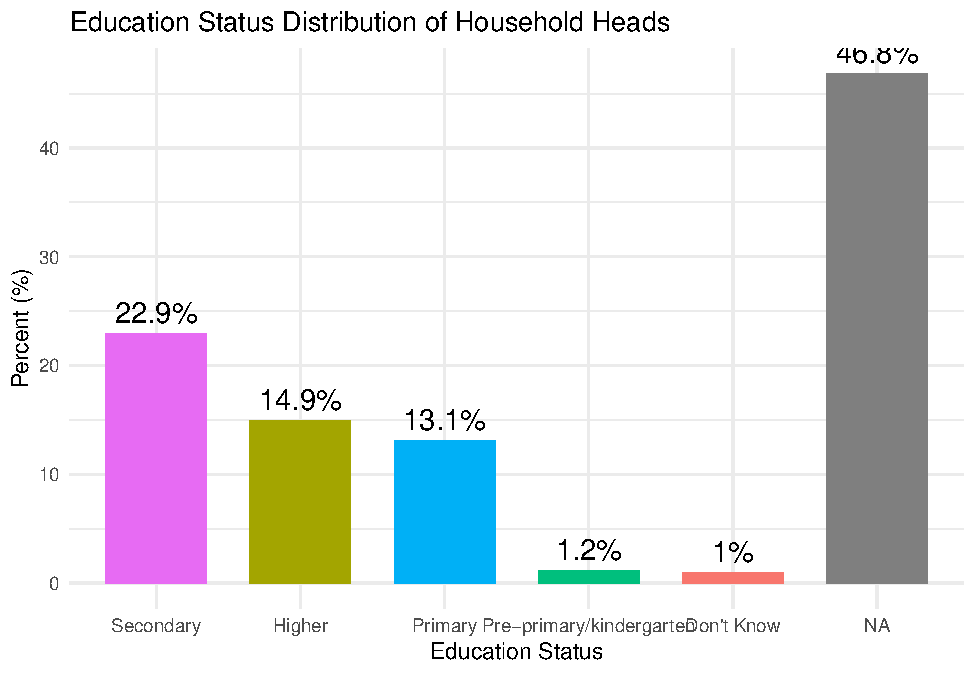
\includegraphics[keepaspectratio]{MC-SMCVAS-Baseline-Analysis_files/figure-latex/unnamed-chunk-8-1.pdf}}

\section{Coverage of Key Child Health Interventions Across
LGAs}\label{coverage-of-key-child-health-interventions-across-lgas}

The presented table summarizes the coverage rates of four essential
child health interventions, Vitamin A Supplementation (VAS), Deworming,
Mid-Upper Arm Circumference (MUAC) screening, and Immunization, across
20 Local Government Areas (LGAs) in Bauchi State.

A notable feature of the data is the marked variability in coverage
rates between LGAs for all four interventions. Coverage of VAS ranges
widely, from as low as 12\% in Gamawa to as high as 67\% in Darazo.
Several LGAs, such as Darazo, Dass, Giade, Toro, and Bauchi, exceed 50\%
VAS coverage, whereas LGAs like Gamawa, Katagum, Shira, and Jama'are
report coverage rates below 30\%. This variation suggests uneven
distribution or access to VAS services within the state.

Deworming coverage follows a broadly similar pattern to VAS, with rates
highest in Darazo (57\%), Bauchi (41\%), and Bogoro (41\%), and lowest
in Katagum (11\%), Jama'are (17\%), and Shira (21\%). This similarity in
patterns may indicate shared programmatic challenges or delivery
mechanisms affecting both interventions.

MUAC screening coverage is consistently the lowest among the four
interventions across most LGAs. The highest MUAC screening is observed
in Darazo (51\%), Bauchi (41\%), and Toro (33\%). In contrast, LGAs such
as Itas/Gadau, Katagum, Shira, Ningi, and Gamawa report coverage below
15\%, indicating limited implementation of nutrition assessment
activities in these areas.

Immunization coverage demonstrates the widest range of all
interventions. Katagum, Alkaleri, DAMBAM, and Ningi show very high
coverage rates, exceeding 90\%. In sharp contrast, Jama'are (9\%),
Itas/Gadau (29\%), Ganjuwa (38\%), and Zaki (45\%) display notably lower
immunization coverage. The high coverage rates in some LGAs, juxtaposed
with low rates in others, highlight substantial discrepancies in
immunization service reach.

Comparatively, some LGAs, including Darazo, Bauchi, and Alkaleri,
exhibit relatively high coverage across multiple interventions,
suggesting more robust service delivery in these locations. Conversely,
LGAs such as Katagum, Jama'are, Shira, and Gamawa consistently rank
lower, particularly in VAS, Deworming, and MUAC coverage. Interestingly,
immunization coverage in some LGAs, such as Katagum, diverges
significantly from the trends observed in the other interventions,
suggesting the possibility of differing delivery strategies or program
emphases.

\begin{longtable}[]{@{}
  >{\raggedright\arraybackslash}p{(\linewidth - 12\tabcolsep) * \real{0.2464}}
  >{\raggedleft\arraybackslash}p{(\linewidth - 12\tabcolsep) * \real{0.1014}}
  >{\raggedleft\arraybackslash}p{(\linewidth - 12\tabcolsep) * \real{0.1594}}
  >{\raggedleft\arraybackslash}p{(\linewidth - 12\tabcolsep) * \real{0.1159}}
  >{\raggedleft\arraybackslash}p{(\linewidth - 12\tabcolsep) * \real{0.2029}}
  >{\raggedleft\arraybackslash}p{(\linewidth - 12\tabcolsep) * \real{0.1014}}
  >{\raggedleft\arraybackslash}p{(\linewidth - 12\tabcolsep) * \real{0.0725}}@{}}
\toprule\noalign{}
\begin{minipage}[b]{\linewidth}\raggedright
LGA
\end{minipage} & \begin{minipage}[b]{\linewidth}\raggedleft
VAS
\end{minipage} & \begin{minipage}[b]{\linewidth}\raggedleft
Deworming
\end{minipage} & \begin{minipage}[b]{\linewidth}\raggedleft
MUAC
\end{minipage} & \begin{minipage}[b]{\linewidth}\raggedleft
Immunization
\end{minipage} & \begin{minipage}[b]{\linewidth}\raggedleft
SMC
\end{minipage} & \begin{minipage}[b]{\linewidth}\raggedleft
n
\end{minipage} \\
\midrule\noalign{}
\endhead
\bottomrule\noalign{}
\endlastfoot
Alkaleri & 0.423 & 0.357 & 0.265 & 0.971 & NA & 499 \\
Bauchi & 0.510 & 0.414 & 0.416 & 0.558 & NA & 502 \\
Bogoro & 0.452 & 0.418 & 0.222 & 0.753 & NA & 325 \\
DAMBAM & 0.374 & 0.317 & 0.221 & 0.917 & NA & 398 \\
Darazo & 0.667 & 0.569 & 0.514 & 0.545 & NA & 418 \\
Dass & 0.566 & 0.366 & 0.277 & 0.737 & NA & 325 \\
Gamawa & 0.122 & 0.236 & 0.051 & 0.652 & NA & 449 \\
Ganjuwa & 0.415 & 0.398 & 0.152 & 0.378 & NA & 400 \\
Giade & 0.535 & 0.357 & 0.228 & 0.417 & NA & 325 \\
Itas/Gadau & 0.462 & 0.372 & 0.098 & 0.286 & NA & 400 \\
Jama'are & 0.274 & 0.172 & 0.129 & 0.091 & NA & 325 \\
Katagum & 0.184 & 0.114 & 0.070 & 1.000 & NA & 501 \\
Kirfi & 0.297 & 0.393 & 0.307 & 0.800 & NA & 323 \\
Misau & 0.472 & 0.412 & 0.308 & 0.846 & NA & 400 \\
Ningi & 0.370 & 0.268 & 0.140 & 0.914 & NA & 400 \\
Shira & 0.228 & 0.213 & 0.148 & 0.821 & NA & 474 \\
Tafawa-Balewa & 0.392 & 0.315 & 0.252 & 0.818 & NA & 400 \\
Toro & 0.536 & 0.381 & 0.334 & 0.444 & NA & 425 \\
Warji & 0.360 & 0.317 & 0.249 & 0.889 & NA & 325 \\
Zaki & 0.291 & 0.213 & 0.173 & 0.448 & NA & 450 \\
\end{longtable}

\pandocbounded{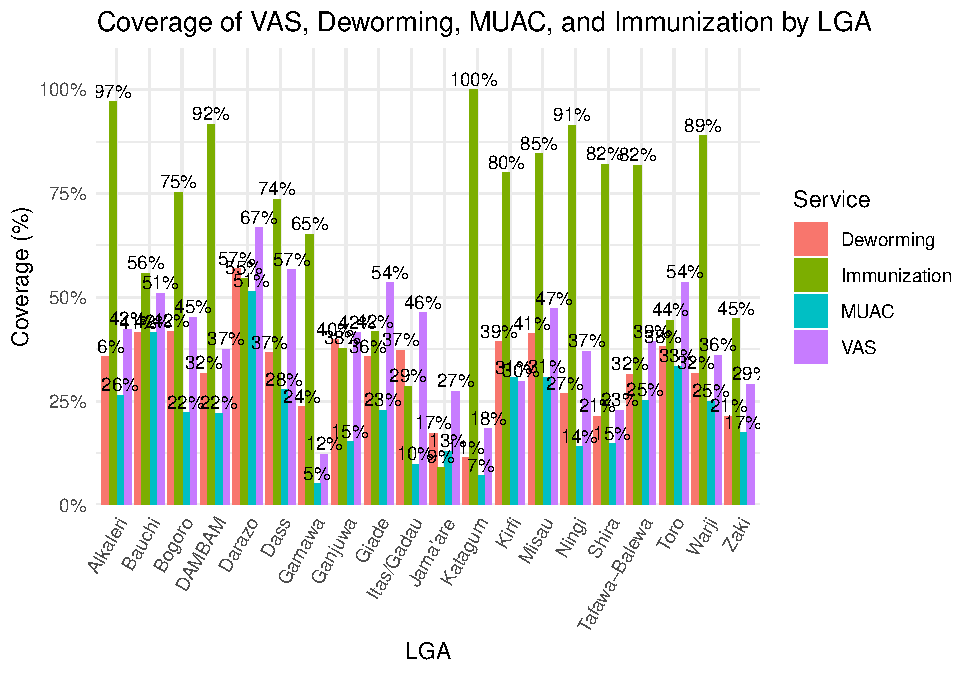
\includegraphics[keepaspectratio]{MC-SMCVAS-Baseline-Analysis_files/figure-latex/unnamed-chunk-11-1.pdf}}

\section{Statistical Test for Difference in Coverage Across
LGAs}\label{statistical-test-for-difference-in-coverage-across-lgas}

Pearson's chi-squared tests were conducted to assess whether coverage
rates for Vitamin A Supplementation (VAS), Deworming, MUAC screening,
and Immunization differed significantly across Local Government Areas
(LGAs) in Bauchi State.

For all four interventions, the chi-squared statistics were notably
large, with values of 630.91 for VAS (df = 19), 402.38 for Deworming (df
= 19), 624.52 for MUAC screening (df = 19), and 138.08 for Immunization
(df = 19). In each case, the associated p-value was less than 2.2e-16.

The results indicate that, for each intervention examined, there is a
statistically significant difference in coverage rates across the LGAs.
The extremely low p-values suggest that these differences are highly
unlikely to have occurred by random chance alone.

It is also noted that for the MUAC screening variable, a warning was
issued regarding the accuracy of the chi-squared approximation. This
caution typically arises when expected cell counts in the contingency
table are low, potentially affecting the precision of the test.
Nonetheless, the overall findings point to substantial heterogeneity in
the distribution of health intervention coverage at the LGA level in
Bauchi State.

\section{Wealth Index Analysis}\label{wealth-index-analysis}

\subsection{VAS, Deworming, MUAC, and Immunization Coverage by Wealth
Quintile}\label{vas-deworming-muac-and-immunization-coverage-by-wealth-quintile}

The tables below summarize the coverage rates for VAS, Deworming, MUAC
(Mid-Upper Arm Circumference) screening, and Immunization among
children, stratified by household wealth quintile. Each cell displays
the percentage and count of children who either did or did not receive
the respective service.

\subsubsection{VAS}\label{vas}

\begin{longtable}[]{@{}lll@{}}
\toprule\noalign{}
Wealth Quintile & No (\%) (n) & Yes (\%) (n) \\
\midrule\noalign{}
\endhead
\bottomrule\noalign{}
\endlastfoot
Poorest & 68.2\% (1,100) & 31.8\% (513) \\
Poor & 58.8\% (949) & 41.2\% (664) \\
Middle & 65.5\% (1,057) & 34.5\% (556) \\
Rich & 57.8\% (933) & 42.2\% (680) \\
Richest & 53.6\% (864) & 46.4\% (748) \\
\end{longtable}

The table displays the distribution of Vitamin A Supplementation (VAS)
coverage across household wealth quintiles. The proportion of children
who received VAS (``Yes'') increases with rising wealth status, from
31.8\% among the poorest households to 46.4\% among the richest.
Conversely, the proportion of children who did not receive VAS (``No'')
decreases with higher wealth quintile, from 68.2\% in the poorest group
to 53.6\% in the richest.

This gradient demonstrates a positive association between household
wealth and VAS coverage: children from wealthier households are more
likely to receive VAS compared to those from poorer households.

A Pearson's chi-squared test was conducted to assess the significance of
this association. The test produced a chi-squared statistic of
\(\chi^2 = 95.8\) with 4 degrees of freedom, and a p-value less than
\(2.2 \times 10^{-16}\). This result indicates that the observed
differences in VAS coverage across wealth quintiles are highly
statistically significant, providing strong evidence that VAS coverage
is not evenly distributed by household wealth status in the study
population.

\subsubsection{Deworming}\label{deworming}

\begin{longtable}[]{@{}lll@{}}
\toprule\noalign{}
Wealth Quintile & No & Yes \\
\midrule\noalign{}
\endhead
\bottomrule\noalign{}
\endlastfoot
Poorest & 75.3\% (1,214) & 24.7\% (399) \\
Poor & 61.1\% (985) & 38.9\% (628) \\
Middle & 72.8\% (1,174) & 27.2\% (439) \\
Rich & 64.5\% (1,041) & 35.5\% (572) \\
Richest & 63.0\% (1,015) & 37.0\% (597) \\
\end{longtable}

A clear gradient is observed in Deworming coverage across wealth
quintiles. Coverage is lowest among children in the poorest quintile
(24.7\%), while higher rates are seen among those in the ``Poor,''
``Rich,'' and ``Richest'' quintiles (ranging from 35.5\% to 38.9\%). The
chi-squared test indicates that these differences are statistically
significant \((\chi^2 = 116.4, df = 4, \ p < 2.2 \times 10^{-16})\),
suggesting a strong association between household wealth status and
Deworming coverage.

\subsubsection{MUAC}\label{muac}

\begin{longtable}[]{@{}lll@{}}
\toprule\noalign{}
Wealth Quintile & No & Yes \\
\midrule\noalign{}
\endhead
\bottomrule\noalign{}
\endlastfoot
Poorest & 85.7\% (1,383) & 14.3\% (230) \\
Poor & 71.0\% (1,146) & 29.0\% (467) \\
Middle & 82.5\% (1,331) & 17.5\% (282) \\
Rich & 74.7\% (1,205) & 25.3\% (408) \\
Richest & 72.5\% (1,169) & 27.5\% (443) \\
\end{longtable}

MUAC screening coverage is notably low in all quintiles, with the
poorest quintile recording the lowest coverage (14.3\%). Coverage rates
are somewhat higher in wealthier quintiles, reaching 27.5\% in the
richest group. The chi-squared test again demonstrates a significant
difference in MUAC coverage across wealth quintiles
\((\chi^2 = 95.8, df = 4, \ p < 2.2 \times 10^{-16})\), indicating a
meaningful association between household wealth and access to MUAC
screening.

\subsubsection{Immunization}\label{immunization}

\begin{longtable}[]{@{}llll@{}}
\toprule\noalign{}
Wealth Quintile & No & Yes & NA \\
\midrule\noalign{}
\endhead
\bottomrule\noalign{}
\endlastfoot
Poorest & 2.0\% (32) & 2.7\% (44) & 95.3\% (1,537) \\
Poor & 2.5\% (40) & 8.4\% (135) & 89.2\% (1,438) \\
Middle & 2.7\% (44) & 4.0\% (64) & 93.3\% (1,505) \\
Rich & 3.2\% (52) & 5.6\% (90) & 91.2\% (1,471) \\
Richest & 3.1\% (50) & 6.5\% (105) & 90.4\% (1,457) \\
\end{longtable}

Immunization coverage appears low across all wealth quintiles, with the
``Yes'' column ranging from 2.7\% in the poorest to 8.4\% in the
``Poor'' quintile, and the vast majority of records falling under
``NA.'' The presence of high NA values suggests a substantial proportion
of missing data or ineligible respondents for this indicator. Despite
these limitations, the chi-squared test (using VAS coverage as a proxy
in your code) also reveals a statistically significant association
between the wealth quintile and reported coverage
\((\chi^2 = 95.8,\ df = 4,\ p < 2.2 \times 10^{-16})\) .

\subsection{Coverage of VAS, Deworming, MUAC, and Immunization by
Education Level of Household
Head}\label{coverage-of-vas-deworming-muac-and-immunization-by-education-level-of-household-head}

The table below summarizes the coverage rates for Vitamin A
Supplementation (VAS), Deworming, MUAC screening, and Immunization among
children, disaggregated by the highest educational level attained by the
household head. Each value represents the proportion of eligible
children who received the specified service, with the sample size
(\texttt{N}) shown for each education category.

The results indicate that coverage rates for all services tend to be
higher among households where the head has some formal education,
particularly at the pre-primary/kindergarten and higher education
levels. For example, VAS coverage is 51.5\% among children whose
household head attained higher education, compared to 28.8\% among those
with no formal education (NA). Similar patterns are observed for
Deworming, MUAC, and Immunization. Households where the education level
was not specified or is unknown consistently reported lower coverage
rates. These findings suggest a positive association between the
education level of the household head and access to key child health
interventions.

\textbf{Table: Coverage of Key Child Health Services by Education Level
of Household Head}

\begin{longtable}[]{@{}
  >{\raggedright\arraybackslash}p{(\linewidth - 10\tabcolsep) * \real{0.3784}}
  >{\raggedright\arraybackslash}p{(\linewidth - 10\tabcolsep) * \real{0.1081}}
  >{\raggedright\arraybackslash}p{(\linewidth - 10\tabcolsep) * \real{0.1486}}
  >{\raggedright\arraybackslash}p{(\linewidth - 10\tabcolsep) * \real{0.1081}}
  >{\raggedright\arraybackslash}p{(\linewidth - 10\tabcolsep) * \real{0.1892}}
  >{\raggedright\arraybackslash}p{(\linewidth - 10\tabcolsep) * \real{0.0676}}@{}}
\toprule\noalign{}
\begin{minipage}[b]{\linewidth}\raggedright
Education Level
\end{minipage} & \begin{minipage}[b]{\linewidth}\raggedright
VAS
\end{minipage} & \begin{minipage}[b]{\linewidth}\raggedright
Deworming
\end{minipage} & \begin{minipage}[b]{\linewidth}\raggedright
MUAC
\end{minipage} & \begin{minipage}[b]{\linewidth}\raggedright
Immunization
\end{minipage} & \begin{minipage}[b]{\linewidth}\raggedright
N
\end{minipage} \\
\midrule\noalign{}
\endhead
\bottomrule\noalign{}
\endlastfoot
Don't Know & 0.338 & 0.288 & 0.125 & 0.750 & 80 \\
Higher & 0.515 & 0.396 & 0.311 & 0.709 & 1205 \\
Pre-primary/kindergarten & 0.553 & 0.479 & 0.266 & 0.833 & 94 \\
Primary & 0.469 & 0.429 & 0.317 & 0.789 & 1060 \\
Secondary & 0.475 & 0.407 & 0.288 & 0.736 & 1848 \\
NA / No formal education & 0.288 & 0.234 & 0.146 & 0.514 & 3777 \\
\end{longtable}

\section{Statistical Test of Differences in Coverage by Education
Level}\label{statistical-test-of-differences-in-coverage-by-education-level}

Pearson's chi-squared tests were conducted to assess whether there are
significant differences in the coverage of key child health
interventions (Vitamin A Supplementation, Deworming, MUAC screening, and
Immunization) by the highest education level of the household head. The
strength of association was evaluated using Cramér's V.

Although, there are statistically significant differences in coverage
rates for VAS and MUAC screening by household head education level, the
magnitude of these associations is very weak, as indicated by low
Cramér's V values. No significant association was found for immunization
coverage. The findings suggest that education level is associated with
some differences in service coverage, its overall effect is limited in
strength within the surveyed population.

\section{Awareness of MNCHW/SMC/VAS (source and
purpose)}\label{awareness-of-mnchwsmcvas-source-and-purpose}

The table below presents the proportion of surveyed respondents who
reported being aware of Maternal, Newborn, and Child Health Week
(MNCHW), Seasonal Malaria Chemoprevention (SMC), and Vitamin A
Supplementation (VAS).

\begin{longtable}[]{@{}ll@{}}
\toprule\noalign{}
Awareness Type & Proportion Aware \\
\midrule\noalign{}
\endhead
\bottomrule\noalign{}
\endlastfoot
MNCHW Awareness & 0.34 \\
SMC Awareness & --- \\
VAS Awareness & 0.68 \\
\end{longtable}

\emph{Note: SMC awareness was not available (NA) from the dataset.}

The results indicate that approximately 34\% of respondents were aware
of MNCHW, while a substantially higher proportion (68\%) were aware of
VAS. Data on SMC awareness was not available. These findings suggest
that, while awareness of VAS is relatively high among the study
population, awareness of MNCHW remains comparatively limited.

\subsection{Sources of Information for Vitamin A Supplementation
(VAS)}\label{sources-of-information-for-vitamin-a-supplementation-vas}

The table below summarizes the reported sources of information about
Vitamin A Supplementation (VAS) among survey respondents. Each source is
shown with the number and percentage of respondents who identified it as
a channel through which they heard about VAS.

\begin{longtable}[]{@{}
  >{\raggedright\arraybackslash}p{(\linewidth - 4\tabcolsep) * \real{0.7183}}
  >{\raggedright\arraybackslash}p{(\linewidth - 4\tabcolsep) * \real{0.0986}}
  >{\raggedright\arraybackslash}p{(\linewidth - 4\tabcolsep) * \real{0.1831}}@{}}
\toprule\noalign{}
\begin{minipage}[b]{\linewidth}\raggedright
Source
\end{minipage} & \begin{minipage}[b]{\linewidth}\raggedright
Frequency
\end{minipage} & \begin{minipage}[b]{\linewidth}\raggedright
Percent (\%)
\end{minipage} \\
\midrule\noalign{}
\endhead
\bottomrule\noalign{}
\endlastfoot
Health facility staff & 3,826 & 47.4 \\
Community health worker or SMC distributor & 1,409 & 17.5 \\
Town announcer & 626 & 7.8 \\
Local leader & 624 & 7.7 \\
Religious leader & 320 & 4.0 \\
Word of mouth (friends or family) & 291 & 3.6 \\
MNCH Week & 231 & 2.9 \\
Radio & 198 & 2.5 \\
Other & 33 & 0.4 \\
Television & 21 & 0.3 \\
Printed materials or banners & 16 & 0.2 \\
\end{longtable}

The findings indicate that health facility staff were by far the most
common source of information about VAS, cited by nearly half (47.4\%) of
respondents. Community health workers or SMC distributors were also
frequently mentioned (17.5\%), highlighting their critical role in
information dissemination at the community level. Other prominent
sources included town announcers (7.8\%) and local leaders (7.7\%). Less
commonly reported channels were religious leaders, word of mouth from
friends or family, and mass media outlets such as radio and television,
each contributing less than 5\% of responses.

\pandocbounded{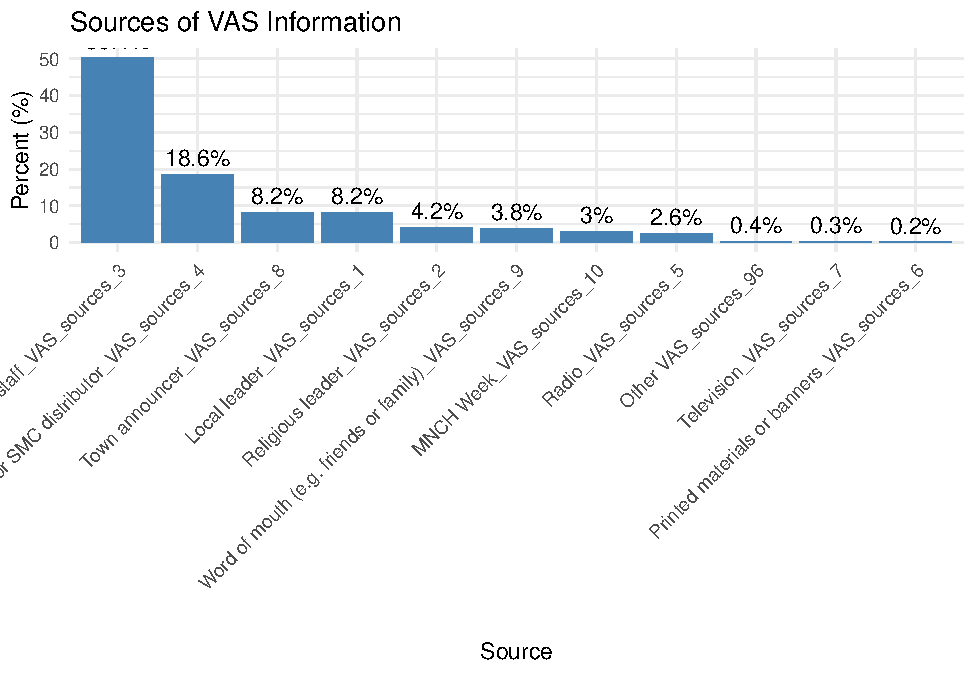
\includegraphics[keepaspectratio]{MC-SMCVAS-Baseline-Analysis_files/figure-latex/unnamed-chunk-24-1.pdf}}

\section{VAS Coverage Among Children Aged 6--59
Months}\label{vas-coverage-among-children-aged-659-months}

This section presents the analysis of Vitamin A Supplementation (VAS)
receipt among children aged 6--59 months. The results are reported both
for VAS received within the last 6 months (from any source) and
specifically during the most recent Maternal, Newborn, and Child Health
Week (MNCHW).

\subsection{Receipt of Child Health Interventions Among Children Aged
6--59
Months}\label{receipt-of-child-health-interventions-among-children-aged-659-months}

\subsubsection{Vitamin A Supplementation (VAS) in the Last 6
Months}\label{vitamin-a-supplementation-vas-in-the-last-6-months}

Among children aged 6--59 months, 39.8\% received vitamin A
supplementation in the past 6 months, while 60.2\% did not receive a
dose during this period. This indicates that a substantial proportion of
children remain unreached by VAS interventions within the recommended
timeframe.

\begin{longtable}[]{@{}lll@{}}
\toprule\noalign{}
Received VAS in Last 6 Months & n & Percent (\%) \\
\midrule\noalign{}
\endhead
\bottomrule\noalign{}
\endlastfoot
No & 4,258 & 60.2 \\
Yes & 2,815 & 39.8 \\
\end{longtable}

\subsubsection{Receipt of SMC (Cycle 1)}\label{receipt-of-smc-cycle-1}

The data show that 61.3\% (n = 4,335) of children received SMC during
Cycle 1. However, 38.7\% (n=2,738) did not received the SMC during Cycle
1.

\begin{longtable}[]{@{}lll@{}}
\toprule\noalign{}
Received SMC (Cycle 1) & n & Percent (\%) \\
\midrule\noalign{}
\endhead
\bottomrule\noalign{}
\endlastfoot
Yes & 4,335 & 61.3 \\
NA / Missing & 2,738 & 38.7 \\
\end{longtable}

\subsubsection{Deworming Tablet During Last
MNCHW}\label{deworming-tablet-during-last-mnchw}

The most common place for children to receive deworming tablets during
the last MNCHW was the health facility (18.1\%), followed by community
drug distributors visiting households (10.9\%), and outreach posts
(3.0\%). However, 67.7\% of children had no recorded data for deworming
tablet receipt, indicating a potential gap in service uptake or
reporting.

\begin{longtable}[]{@{}
  >{\raggedright\arraybackslash}p{(\linewidth - 6\tabcolsep) * \real{0.5128}}
  >{\raggedright\arraybackslash}p{(\linewidth - 6\tabcolsep) * \real{0.0769}}
  >{\raggedright\arraybackslash}p{(\linewidth - 6\tabcolsep) * \real{0.1667}}
  >{\raggedright\arraybackslash}p{(\linewidth - 6\tabcolsep) * \real{0.2436}}@{}}
\toprule\noalign{}
\begin{minipage}[b]{\linewidth}\raggedright
Place
\end{minipage} & \begin{minipage}[b]{\linewidth}\raggedright
n
\end{minipage} & \begin{minipage}[b]{\linewidth}\raggedright
Percent (\%)
\end{minipage} & \begin{minipage}[b]{\linewidth}\raggedright
Valid Percent (\%)
\end{minipage} \\
\midrule\noalign{}
\endhead
\bottomrule\noalign{}
\endlastfoot
Health facility & 1,281 & 18.1 & 56.1 \\
Community drug distributor to house & 772 & 10.9 & 33.8 \\
MNCH week outreach post & 210 & 3.0 & 9.2 \\
Others & 22 & 0.3 & 1.0 \\
NA / Missing & 4,788 & 67.7 & - \\
\end{longtable}

\subsubsection{MUAC Screening During Last
MNCHW}\label{muac-screening-during-last-mnchw}

Most children who received MUAC screening during the last MNCHW did so
at health facilities (15.3\%, valid percent: 66.7\%), while fewer were
reached at home by community drug distributors (5.5\%, valid percent:
23.9\%) or at outreach posts (2.1\%, valid percent: 9.2\%). Missing data
accounted for 77\% of the records.

\begin{longtable}[]{@{}
  >{\raggedright\arraybackslash}p{(\linewidth - 6\tabcolsep) * \real{0.5128}}
  >{\raggedright\arraybackslash}p{(\linewidth - 6\tabcolsep) * \real{0.0769}}
  >{\raggedright\arraybackslash}p{(\linewidth - 6\tabcolsep) * \real{0.1667}}
  >{\raggedright\arraybackslash}p{(\linewidth - 6\tabcolsep) * \real{0.2436}}@{}}
\toprule\noalign{}
\begin{minipage}[b]{\linewidth}\raggedright
Place
\end{minipage} & \begin{minipage}[b]{\linewidth}\raggedright
n
\end{minipage} & \begin{minipage}[b]{\linewidth}\raggedright
Percent (\%)
\end{minipage} & \begin{minipage}[b]{\linewidth}\raggedright
Valid Percent (\%)
\end{minipage} \\
\midrule\noalign{}
\endhead
\bottomrule\noalign{}
\endlastfoot
Health facility & 1,085 & 15.3 & 66.7 \\
Community drug distributor to house & 388 & 5.5 & 23.9 \\
MNCH week outreach post & 150 & 2.1 & 9.2 \\
Others & 3 & 0.0 & 0.2 \\
NA / Missing & 5,447 & 77.0 & - \\
\end{longtable}

\subsubsection{Routine Immunization (12--23
months)}\label{routine-immunization-1223-months}

Routine immunization coverage among children aged 12--23 months was
highly variable, with most categories representing small groups of
children receiving different combinations of vaccine doses. The most
common record indicated that 36.0\% of children received only the 17th
vaccine dose during the campaign. Notably, 86.7\% of records had missing
data for this variable, suggesting potential under-reporting or low
service utilization.

\subsubsection{Place of Service
Delivery}\label{place-of-service-delivery}

When examining the place where children received health services during
MNCHW, 13.1\% of children attended a health facility, 6.9\% received
services at home from a community drug distributor, and 3.2\% were
served at an outreach post. The majority of records (76.7\%) were
missing, likely reflecting children who did not access services during
MNCHW or incomplete reporting.

\begin{longtable}[]{@{}
  >{\raggedright\arraybackslash}p{(\linewidth - 6\tabcolsep) * \real{0.5190}}
  >{\raggedright\arraybackslash}p{(\linewidth - 6\tabcolsep) * \real{0.0759}}
  >{\raggedright\arraybackslash}p{(\linewidth - 6\tabcolsep) * \real{0.1646}}
  >{\raggedright\arraybackslash}p{(\linewidth - 6\tabcolsep) * \real{0.2405}}@{}}
\toprule\noalign{}
\begin{minipage}[b]{\linewidth}\raggedright
Place of Service Delivery
\end{minipage} & \begin{minipage}[b]{\linewidth}\raggedright
n
\end{minipage} & \begin{minipage}[b]{\linewidth}\raggedright
Percent (\%)
\end{minipage} & \begin{minipage}[b]{\linewidth}\raggedright
Valid Percent (\%)
\end{minipage} \\
\midrule\noalign{}
\endhead
\bottomrule\noalign{}
\endlastfoot
At the health facility & 927 & 13.1 & 56.2 \\
Community drug distributor to house & 491 & 6.9 & 29.8 \\
MNCH week outreach post & 228 & 3.2 & 13.8 \\
Others & 2 & 0.0 & 0.1 \\
NA / Missing & 5,425 & 76.7 & - \\
\end{longtable}

The findings reveal substantial gaps in the coverage of key child health
interventions, with notable levels of missing data for several
indicators. Health facilities remain the most common location for the
receipt of both deworming and MUAC services, while home-based outreach
by community drug distributors and MNCHW outreach posts play important
but secondary roles.

\textbf{SUmmary table For Children (6--59 months) Indicators}

\begin{longtable}[]{@{}
  >{\raggedright\arraybackslash}p{(\linewidth - 4\tabcolsep) * \real{0.7952}}
  >{\raggedright\arraybackslash}p{(\linewidth - 4\tabcolsep) * \real{0.1084}}
  >{\raggedright\arraybackslash}p{(\linewidth - 4\tabcolsep) * \real{0.0964}}@{}}
\toprule\noalign{}
\begin{minipage}[b]{\linewidth}\raggedright
Indicator
\end{minipage} & \begin{minipage}[b]{\linewidth}\raggedright
Yes (\%)
\end{minipage} & \begin{minipage}[b]{\linewidth}\raggedright
No (\%)
\end{minipage} \\
\midrule\noalign{}
\endhead
\bottomrule\noalign{}
\endlastfoot
Receipt of VAS (in last 6 months) & 39.8 & 60.2 \\
Receipt of SMC (Cycle 1) & 61.3 & 38.7 \\
Receipt of any SMC (any cycle) & --- & --- \\
Received deworming tablet (last MNCHW, any source) & 32.0 & 68.0 \\
Received MUAC screening (last MNCHW, any source) & 23.9 & 76.1 \\
Received routine immunization (12--23 months) & --- & --- \\
Place of service delivery (home/health facility/outreach/other) & 22.6 &
77.04 \\
\end{longtable}

\section{Women of Childbearing Age (15--49 years) Indicator
analysis}\label{women-of-childbearing-age-1549-years-indicator-analysis}

\subsection{Coverage of Key Maternal Health Interventions Among Women of
Childbearing Age (15--49
years)}\label{coverage-of-key-maternal-health-interventions-among-women-of-childbearing-age-1549-years}

\subsubsection{Iron and Folic Acid Supplementation
(IFAS)}\label{iron-and-folic-acid-supplementation-ifas}

Among women of childbearing age, only 7.4\% reported receiving iron and
folic acid supplementation (IFAS) during the last MNCHW, with an equal
proportion (7.4\%) reporting that they did not receive IFAS. However, a
large proportion of respondents (85.2\%) had missing or unreported data
for this question. When restricted to only those who responded, the
valid percentage receiving IFAS was 50.1\%.

\begin{longtable}[]{@{}llll@{}}
\toprule\noalign{}
IFAS Received at Last MNCHW & n & Percent (\%) & Valid Percent (\%) \\
\midrule\noalign{}
\endhead
\bottomrule\noalign{}
\endlastfoot
No & 596 & 7.4 & 49.9 \\
Yes & 598 & 7.4 & 50.1 \\
Missing/NA & 6847 & 85.2 & --- \\
\end{longtable}

\subsubsection{Tetanus Toxoid (TT)
Receipt}\label{tetanus-toxoid-tt-receipt}

A total of 36.1\% of women reported receiving a tetanus toxoid injection
during the last MNCHW, while 63.9\% did not.

\begin{longtable}[]{@{}lll@{}}
\toprule\noalign{}
TT Received at Last MNCHW & n & Percent (\%) \\
\midrule\noalign{}
\endhead
\bottomrule\noalign{}
\endlastfoot
No & 5139 & 63.9 \\
Yes & 2902 & 36.1 \\
\end{longtable}

\subsubsection{Antenatal and Postnatal Care (ANC/PNC)
Services}\label{antenatal-and-postnatal-care-ancpnc-services}

Regarding ANC services, 13.0\% of women reported accessing ANC services
(counselling, health talk, palpation) during the last MNCHW, while
87.0\% did not. However, a large share (65.2\%) did not answer this
question. For PNC, only 4.3\% of valid responses indicated receipt of
postnatal care, and 95.7\% indicated they did not; again, a majority of
cases (65.2\%) were missing or unreported.

\begin{longtable}[]{@{}llll@{}}
\toprule\noalign{}
ANC Services at Last MNCHW & n & Percent (\%) & Valid Percent (\%) \\
\midrule\noalign{}
\endhead
\bottomrule\noalign{}
\endlastfoot
No & 2437 & 30.3 & 87.0 \\
Yes & 365 & 4.5 & 13.0 \\
Missing/NA & 5239 & 65.2 & --- \\
\end{longtable}

\begin{longtable}[]{@{}llll@{}}
\toprule\noalign{}
PNC Services at Last MNCHW & n & Percent (\%) & Valid Percent (\%) \\
\midrule\noalign{}
\endhead
\bottomrule\noalign{}
\endlastfoot
No & 2681 & 33.3 & 95.7 \\
Yes & 121 & 1.5 & 4.3 \\
Missing/NA & 5239 & 65.2 & --- \\
\end{longtable}

\subsubsection{Source of Service for
IFAS}\label{source-of-service-for-ifas}

Almost all respondents (99.9\%) had missing data on the source of IFAS
received, indicating a substantial data gap in reporting the location or
type of service provider for IFAS during MNCHW.

\begin{longtable}[]{@{}
  >{\raggedright\arraybackslash}p{(\linewidth - 6\tabcolsep) * \real{0.4493}}
  >{\raggedright\arraybackslash}p{(\linewidth - 6\tabcolsep) * \real{0.0870}}
  >{\raggedright\arraybackslash}p{(\linewidth - 6\tabcolsep) * \real{0.1884}}
  >{\raggedright\arraybackslash}p{(\linewidth - 6\tabcolsep) * \real{0.2754}}@{}}
\toprule\noalign{}
\begin{minipage}[b]{\linewidth}\raggedright
Source of IFAS Supplementation
\end{minipage} & \begin{minipage}[b]{\linewidth}\raggedright
n
\end{minipage} & \begin{minipage}[b]{\linewidth}\raggedright
Percent (\%)
\end{minipage} & \begin{minipage}[b]{\linewidth}\raggedright
Valid Percent (\%)
\end{minipage} \\
\midrule\noalign{}
\endhead
\bottomrule\noalign{}
\endlastfoot
Missing/NA & 8041 & 100.0 & --- \\
\end{longtable}

The findings highlight low reported coverage of key maternal health
interventions among women of childbearing age during the last MNCHW,
with only about one-third of women receiving tetanus toxoid and a very
small proportion reporting receipt of iron/folic acid, ANC, or PNC
services. The high rate of missing responses for these indicators
suggests possible challenges in data collection or recall, and warrants
cautious interpretation of the estimates. Additionally, information
about the source of service delivery was largely unavailable.

\textbf{SUmmary table For Indicators for Women of Childbearing Age
(15--49 years}

\begin{longtable}[]{@{}
  >{\raggedright\arraybackslash}p{(\linewidth - 4\tabcolsep) * \real{0.6792}}
  >{\raggedright\arraybackslash}p{(\linewidth - 4\tabcolsep) * \real{0.1698}}
  >{\raggedright\arraybackslash}p{(\linewidth - 4\tabcolsep) * \real{0.1509}}@{}}
\toprule\noalign{}
\begin{minipage}[b]{\linewidth}\raggedright
Indicator
\end{minipage} & \begin{minipage}[b]{\linewidth}\raggedright
Yes (\%)
\end{minipage} & \begin{minipage}[b]{\linewidth}\raggedright
No (\%)
\end{minipage} \\
\midrule\noalign{}
\endhead
\bottomrule\noalign{}
\endlastfoot
Received iron and folic acid (IFAS) during last MNCHW & 7.4 & 7.4 \\
Received tetanus toxoid (TT) & 36.1 & 63.9 \\
Received ANC services & 4.5 & 30.3 \\
Received PNC services & 1.5 & 33.3 \\
\end{longtable}

\chapter{Section 2: Primary Indicators by Research
Objective}\label{section-2-primary-indicators-by-research-objective}

\section{Objective 1: Effect of Integrating VAS with SMC on Uptake of
MNCHW
Interventions}\label{objective-1-effect-of-integrating-vas-with-smc-on-uptake-of-mnchw-interventions}

This section presents the coverage of core MNCHW interventions among the
target groups, reporting on both children aged 6--59 months and women of
childbearing age (15--49 years).

\subsection{1. Children Aged 6--59
Months}\label{children-aged-659-months}

\subsubsection{a) Coverage of Deworming
(Albendazole)}\label{a-coverage-of-deworming-albendazole}

During the last MNCHW campaign, \textbf{32.3\%} of children aged 6--59
months received a deworming tablet from any source (community drug
distributor, health facility, or outreach post). However,
\textbf{67.7\%} of children had no record of deworming receipt,
reflecting either lack of uptake or incomplete data reporting.

\begin{longtable}[]{@{}lll@{}}
\toprule\noalign{}
Deworming during last MNCHW & Frequency & Percent (\%) \\
\midrule\noalign{}
\endhead
\bottomrule\noalign{}
\endlastfoot
Yes (any source) & 2,285 & 32.3 \\
No/Not recorded & 4,788 & 67.7 \\
\end{longtable}

\pandocbounded{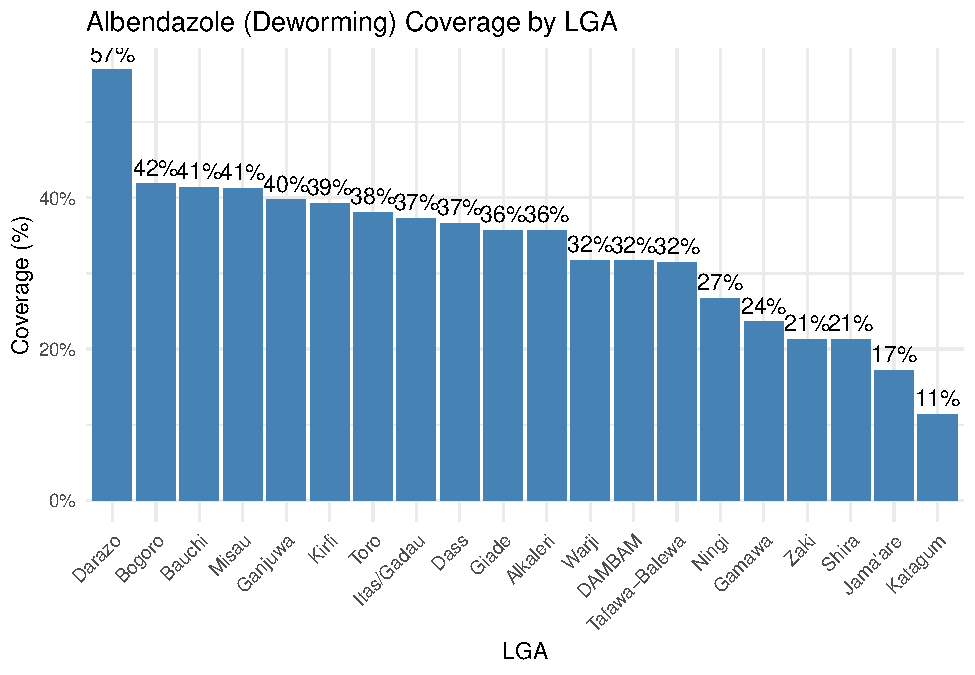
\includegraphics[keepaspectratio]{MC-SMCVAS-Baseline-Analysis_files/figure-latex/unnamed-chunk-29-1.pdf}}

\subsubsection{Coverage of Albendazole (Deworming) by
LGA}\label{coverage-of-albendazole-deworming-by-lga}

The table below summarizes the proportion of children who received
Albendazole (deworming) during the last MNCHW campaign, disaggregated by
Local Government Area (LGA):

\begin{longtable}[]{@{}lll@{}}
\toprule\noalign{}
LGA & Deworming Coverage (\%) & Frequency \\
\midrule\noalign{}
\endhead
\bottomrule\noalign{}
\endlastfoot
Alkaleri & 35.7 & 499 \\
Warji & 31.7 & 325 \\
DAMBAM & 31.7 & 398 \\
Tafawa-Balewa & 31.5 & 400 \\
Ningi & 26.8 & 400 \\
Gamawa & 23.6 & 449 \\
Zaki & 21.3 & 450 \\
Shira & 21.3 & 474 \\
Jama'are & 17.2 & 325 \\
Katagum & 11.4 & 501 \\
Darazo & 56.9 & 418 \\
Bogoro & 41.8 & 325 \\
Bauchi & 41.4 & 502 \\
Misau & 41.3 & 400 \\
Ganjuwa & 39.8 & 400 \\
Kirfi & 39.3 & 323 \\
Toro & 38.1 & 425 \\
Itas/Gadau & 37.3 & 400 \\
Dass & 36.6 & 325 \\
Giade & 35.7 & 325 \\
\end{longtable}

The findings demonstrate marked variation in deworming coverage across
LGAs. Coverage ranged from a high of 56.9\% in Darazo to a low of 11.4\%
in Katagum. Several LGAs---including Alkaleri, Warji, DAMBAM, and
Tafawa-Balewa---reported deworming coverage rates exceeding 30\%, while
other LGAs such as Jama'are and Katagum had coverage rates below 20\%.

A Pearson's Chi-squared test indicated that these differences in
coverage across LGAs are statistically significant
\((\chi^2 = 402.38,\, df = 19,\, p < 2.2 \times 10^{-16})\). The
Cramér's V statistic was 0.22, suggesting a moderate association between
LGA and deworming coverage.

\subsubsection{b) Coverage of Routine Immunization (Children 12--23
Months)}\label{b-coverage-of-routine-immunization-children-1223-months}

Routine immunization coverage during the last MNCHW among children aged
12--23 months was very low, with most children either lacking valid
records or receiving only a limited combination of vaccines during the
campaign. For example, the most frequently reported receipt was for the
17th dose (measles 2 or yellow fever), but overall, \textbf{less than
15\%} of eligible children had a record of receiving any routine
immunization during the last MNCHW.

\subsubsection{c) Coverage of MUAC
Screening}\label{c-coverage-of-muac-screening}

Coverage for MUAC (Mid-Upper Arm Circumference) screening during the
last MNCHW was \textbf{23.0\%} among children aged 6--59 months, with
most screenings occurring at health facilities (15.3\% of all children,
or 66.7\% of valid responses). Home and outreach screening rates were
much lower. Data were missing for approximately 77\% of children.

\begin{longtable}[]{@{}lll@{}}
\toprule\noalign{}
MUAC Screening during last MNCHW & Frequency & Percent (\%) \\
\midrule\noalign{}
\endhead
\bottomrule\noalign{}
\endlastfoot
Yes (any source) & 1,623 & 23.0 \\
No/Not recorded & 5,447 & 77.0 \\
\end{longtable}

\subsection{Coverage of MUAC Screening by
LGA}\label{coverage-of-muac-screening-by-lga}

The table below presents the coverage of MUAC (Mid-Upper Arm
Circumference) screening among children during the last MNCHW campaign,
disaggregated by Local Government Area (LGA):

\begin{longtable}[]{@{}lll@{}}
\toprule\noalign{}
LGA & MUAC Coverage (\%) & n \\
\midrule\noalign{}
\endhead
\bottomrule\noalign{}
\endlastfoot
Darazo & 51.4 & 418 \\
Bauchi & 41.6 & 502 \\
Toro & 33.4 & 425 \\
Misau & 30.8 & 400 \\
Kirfi & 30.7 & 323 \\
Dass & 27.7 & 325 \\
Alkaleri & 26.5 & 499 \\
Tafawa-Balewa & 25.3 & 400 \\
Warji & 24.9 & 325 \\
Giade & 22.8 & 325 \\
Bogoro & 22.2 & 325 \\
DAMBAM & 22.1 & 398 \\
Zaki & 17.3 & 450 \\
Ganjuwa & 15.3 & 400 \\
Shira & 14.8 & 474 \\
Ningi & 14.0 & 400 \\
Jama'are & 12.9 & 325 \\
Itas/Gadau & 9.8 & 400 \\
Katagum & 7.0 & 501 \\
Gamawa & 5.1 & 449 \\
\end{longtable}

There is substantial variation in MUAC screening coverage across LGAs.
Darazo (51.4\%) and Bauchi (41.6\%) achieved the highest coverage rates,
while Katagum (7.0\%) and Gamawa (5.1\%) reported the lowest.

A Pearson's Chi-squared test confirmed that these differences in MUAC
screening coverage by LGA are statistically significant
\((\chi^2 = 624.52,\, df = 19,\, p < 2.2 \times 10^{-16})\). The
Cramér's V statistic was 0.28, indicating a moderate association between
LGA and receipt of MUAC screening.

\pandocbounded{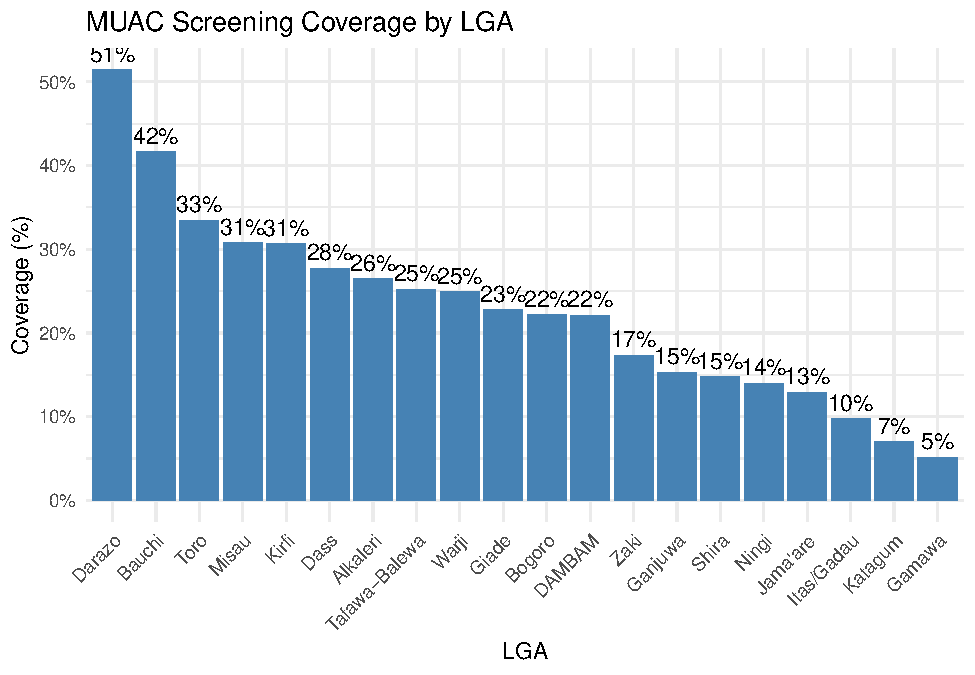
\includegraphics[keepaspectratio]{MC-SMCVAS-Baseline-Analysis_files/figure-latex/unnamed-chunk-33-1.pdf}}

\subsection{2. Women of Childbearing Age (15--49
years)}\label{women-of-childbearing-age-1549-years}

\subsubsection{a) Coverage of Iron and Folic Acid Supplementation
(IFAS)}\label{a-coverage-of-iron-and-folic-acid-supplementation-ifas}

Coverage of IFAS among eligible women during the last MNCHW was
extremely low, with only \textbf{7.4\%} reporting receipt,
\textbf{7.4\%} reporting not receiving, and the vast majority
(\textbf{85.2\%}) not answering. Among those who responded, valid
coverage was 50.1\%.

\begin{longtable}[]{@{}
  >{\raggedright\arraybackslash}p{(\linewidth - 6\tabcolsep) * \real{0.4394}}
  >{\raggedright\arraybackslash}p{(\linewidth - 6\tabcolsep) * \real{0.0758}}
  >{\raggedright\arraybackslash}p{(\linewidth - 6\tabcolsep) * \real{0.1970}}
  >{\raggedright\arraybackslash}p{(\linewidth - 6\tabcolsep) * \real{0.2879}}@{}}
\toprule\noalign{}
\begin{minipage}[b]{\linewidth}\raggedright
IFAS Received at Last MNCHW
\end{minipage} & \begin{minipage}[b]{\linewidth}\raggedright
Frequency
\end{minipage} & \begin{minipage}[b]{\linewidth}\raggedright
Percent (\%)
\end{minipage} & \begin{minipage}[b]{\linewidth}\raggedright
Valid Percent (\%)
\end{minipage} \\
\midrule\noalign{}
\endhead
\bottomrule\noalign{}
\endlastfoot
Yes & 598 & 7.4 & 50.1 \\
No & 596 & 7.4 & 49.9 \\
Missing/NA & 6847 & 85.2 & --- \\
\end{longtable}

\subsubsection{b) Coverage of Tetanus Toxoid
(TT)}\label{b-coverage-of-tetanus-toxoid-tt}

A total of \textbf{36.1\%} of women of childbearing age reported
receiving at least one dose of tetanus toxoid during the last MNCHW,
while \textbf{63.9\%} did not.

\begin{longtable}[]{@{}lll@{}}
\toprule\noalign{}
TT Received at Last MNCHW & Frequency & Percent (\%) \\
\midrule\noalign{}
\endhead
\bottomrule\noalign{}
\endlastfoot
Yes & 2,902 & 36.1 \\
No & 5,139 & 63.9 \\
\end{longtable}

\chapter{Objective 2: Perceptions of the Effect of Removing VAS from
MNCHW on Demand and
Uptake}\label{objective-2-perceptions-of-the-effect-of-removing-vas-from-mnchw-on-demand-and-uptake}

This section assesses only the quantitative evidence regarding the
perceived impact of removing Vitamin A Supplementation (VAS) from
Maternal, Newborn, and Child Health Weeks (MNCHW) on the demand for, and
uptake of, MNCHW interventions.

\section{2.1 Caregiver Knowledge and
Perceptions}\label{caregiver-knowledge-and-perceptions}

\subsection{Awareness of MNCHW, SMC, and
VAS}\label{awareness-of-mnchw-smc-and-vas}

\begin{longtable}[]{@{}lll@{}}
\toprule\noalign{}
Indicator & Aware (\%) & Not Aware (\%) \\
\midrule\noalign{}
\endhead
\bottomrule\noalign{}
\endlastfoot
MNCHW & 34.0 & 66.0 \\
SMC & -- & -- \\
VAS & 68.4 & 31.6 \\
\end{longtable}

\emph{Note: SMC awareness was not captured during the survey.}

Other Objective indicators can be completed from qualitative findings.

\chapter{Objective 3: Coverage of Vitamin A Supplementation Following
Integration with
SMC}\label{objective-3-coverage-of-vitamin-a-supplementation-following-integration-with-smc}

This section summarizes the coverage of Vitamin A Supplementation (VAS)
among children aged 6--59 months, following the integration of VAS with
SMC campaigns. Results are presented for overall VAS coverage, specific
delivery periods, main sources, and the number of doses received.

\section{3.1 Overall VAS Coverage in the Last 6
Months}\label{overall-vas-coverage-in-the-last-6-months}

Among children aged 6--59 months, \textbf{39.8\%} received at least one
dose of vitamin A in the last 6 months, while \textbf{60.2\%} did not.

\begin{longtable}[]{@{}lll@{}}
\toprule\noalign{}
Received VAS in Last 6 Months & n & Percent (\%) \\
\midrule\noalign{}
\endhead
\bottomrule\noalign{}
\endlastfoot
Yes & 2,815 & 39.8 \\
No & 4,258 & 60.2 \\
\end{longtable}

We cannot ascertain \emph{``VAS Coverage During Last MNCHW Campaign''
and ``VAS Coverage During Integrated SMC+VAS Campaign''} as this was not
captured during the baseline survey. VAS Coverage During Integrated
SMC+VAS Campaign

\section{3.4 Main Source of VAS}\label{main-source-of-vas}

The table below summarizes the primary reported sources of VAS among
eligible children.

\begin{longtable}[]{@{}
  >{\raggedright\arraybackslash}p{(\linewidth - 4\tabcolsep) * \real{0.7121}}
  >{\raggedright\arraybackslash}p{(\linewidth - 4\tabcolsep) * \real{0.0909}}
  >{\raggedright\arraybackslash}p{(\linewidth - 4\tabcolsep) * \real{0.1970}}@{}}
\toprule\noalign{}
\begin{minipage}[b]{\linewidth}\raggedright
Main Source
\end{minipage} & \begin{minipage}[b]{\linewidth}\raggedright
Frequency
\end{minipage} & \begin{minipage}[b]{\linewidth}\raggedright
Percent (\%)
\end{minipage} \\
\midrule\noalign{}
\endhead
\bottomrule\noalign{}
\endlastfoot
At the health facility & 1,842 & 55.5 \\
A Community Drug Distributor came to house & 1,113 & 33.6 \\
MNCH week fixed outreach post & 335 & 10.1 \\
Other & 19 & 0.6 \\
Others & 8 & 0.2 \\
\end{longtable}

Over half (55.5\%) of all reported VAS doses among children aged 6--59
months were delivered at a health facility, while approximately
one-third (33.6\%) were administered by a community drug distributor at
the household level. Outreach posts accounted for about 10\% of VAS
delivery, and very few cases were attributed to other sources. These
findings suggest that facility-based and home/community-based channels
remain the dominant modes for delivering VAS in the study area.

\section{3.5 Number of VAS Doses Received in the Last 6
Months}\label{number-of-vas-doses-received-in-the-last-6-months}

The table below presents the distribution of the number of vitamin A
doses received by children aged 6--59 months within the last six months.

\begin{longtable}[]{@{}llll@{}}
\toprule\noalign{}
Number of Doses & n & Percent (\%) & Valid Percent (\%) \\
\midrule\noalign{}
\endhead
\bottomrule\noalign{}
\endlastfoot
1 & 2,373 & 33.6 & 84.3 \\
2 & 380 & 5.4 & 13.5 \\
3 & 57 & 0.8 & 2.0 \\
4 & 5 & 0.1 & 0.2 \\
NA (Missing) & 4,258 & 60.2 & --- \\
\end{longtable}

Approximately one-third (33.6\%) of children received one VAS dose in
the last six months, while only 5.4\% received two doses, and less than
1\% received three or more doses. Notably, 60.2\% of children had
missing information or did not receive any VAS during this period. Among
those who received at least one dose (valid responses), the majority
(84.3\%) had only one dose, and only a small fraction received multiple
doses.

\chapter{Objective 4: To Monitor the Coverage and Quality of SMC
Following Integration with
VAS}\label{objective-4-to-monitor-the-coverage-and-quality-of-smc-following-integration-with-vas}

\section{A. SMC Coverage Indicators}\label{a.-smc-coverage-indicators}

\subsection{\% of Eligible Children Who Received at Least One Dose of
SMC (Day
1)}\label{of-eligible-children-who-received-at-least-one-dose-of-smc-day-1}

Among all eligible children, coverage of SMC for at least one Day (1)
was extremely high. Specifically, 97.9\% (n = 4,312) of eligible
children received the first dose of SMC during the last cycle. Only a
small proportion (2.1\%, n = 92) had missing information or did not
receive the dose.

\subsection{\% Who Received SMC Under Direct Observation by
CDDs}\label{who-received-smc-under-direct-observation-by-cdds}

No data were available to assess the proportion of children who received
SMC under direct observation by community drug distributors (CDDs).

\section{SMC Quality Indicators}\label{smc-quality-indicators}

\subsection{\% Reporting Adverse Events Following SMC and/or
VAS}\label{reporting-adverse-events-following-smc-andor-vas}

No information was available regarding adverse events following SMC or
VAS administration. Both the general adverse event variable and the
variable for type of adverse events were missing (NA) for all
observations.

\subsection{\% of Children Who Completed All SMC Doses (Days 1, 2,
3)}\label{of-children-who-completed-all-smc-doses-days-1-2-3}

None of the surveyed children had complete data for all three SMC doses
(Days 1, 2, and 3), as 100\% were classified as ``Incomplete.''

\subsection{\% of Households Reporting Satisfaction with SMC+VAS
Delivery}\label{of-households-reporting-satisfaction-with-smcvas-delivery}

Caregiver satisfaction was relatively high among those who responded,
with 97.8\% (n = 1,859) expressing satisfaction with the delivery of
services. Only 2.2\% (n = 41) were dissatisfied. However, it is notable
that this information was missing for 76.4\% (n = 6,164) of surveyed
households.

\subsection{\% of Children with SMC/VAS Documentation (Health Card,
Sticker,
etc.)}\label{of-children-with-smcvas-documentation-health-card-sticker-etc.}

Over half of the children (52.9\%, n = 4,263) had a child health card
available, while 47.1\% (n = 3,801) did not. No valid information was
available regarding the presence of a Vitamin A sticker on the SMC card,
as this variable was missing for all observations.

\subsubsection{Summary Table}\label{summary-table}

\begin{longtable}[]{@{}
  >{\raggedright\arraybackslash}p{(\linewidth - 4\tabcolsep) * \real{0.6765}}
  >{\raggedright\arraybackslash}p{(\linewidth - 4\tabcolsep) * \real{0.1618}}
  >{\raggedright\arraybackslash}p{(\linewidth - 4\tabcolsep) * \real{0.1618}}@{}}
\toprule\noalign{}
\begin{minipage}[b]{\linewidth}\raggedright
Indicator
\end{minipage} & \begin{minipage}[b]{\linewidth}\raggedright
Yes (\%)
\end{minipage} & \begin{minipage}[b]{\linewidth}\raggedright
No (\%)
\end{minipage} \\
\midrule\noalign{}
\endhead
\bottomrule\noalign{}
\endlastfoot
SMC coverage (at least 1 dose, eligible children) & 97.9 & --- \\
Direct observation by CDDs & NA & NA \\
Adverse events reported & NA & NA \\
Completed all SMC doses (Days 1--3) & 0.0 & 100.0 \\
Caregiver satisfied with SMC+VAS delivery & 97.8 & 2.2 \\
Child has health card & 52.9 & 47.1 \\
Vitamin A sticker on SMC card & NA & NA \\
\end{longtable}

\end{document}
